\subsection{Entropy and a ``word game`` implementation}

To explain exactly what entropy is, what better way than to create a bot that has to make choices. Because that's exactly what entropy is, a measure of uncertainty.

Word game or Wordle is a game in which you have to find a random word, and each time you make a move, you receive feedback that lets you know whether for each letter 0: it's in the right place, 1: it's not in the right place, 2: it's not present or no longer present in the word. The words we play are defined in a text document (5-letter English words).
We implemented this game in python and created a bot capable of making choices thanks to entropy.
In our case, each letter of the word is a symbol.
In the context where each symbol is independent, the entropy formula is as follows.

$$-\sum p_i \log(p_i)$$

where pi is the probability of symbol i.

For a word, we'll calculate symbol by symbol, the probability that it will appear (i.e. its frequency at that location) and then apply the formula. Finally, we add up each result, giving the word's entropy.
 
Entropy varies between 0 and 1, when using base 2. When it comes to comparing them and making a choice, the one that tends most towards 0 is the most likely. 
For our context: in the list of available words, we calculate and compare the entropy of each word. Then we use the word with the highest entropy to play and get the next feedback (using the maximum entropy allow us to test the widest sample). 

This process makes it possible to make the best possible choice when feedback is already available. But what about the first choice? We have several options for several results. 

\begin{enumerate}
    \item Calculate the entropy of each word in the complete list, then select the word with the highest entropy.
    \item Put each letter where its frequency is highest.
    \item Calculate the "pairs" of symbols most repeated at each location.
\end{enumerate}

\begin{figure}[!h]
\centering
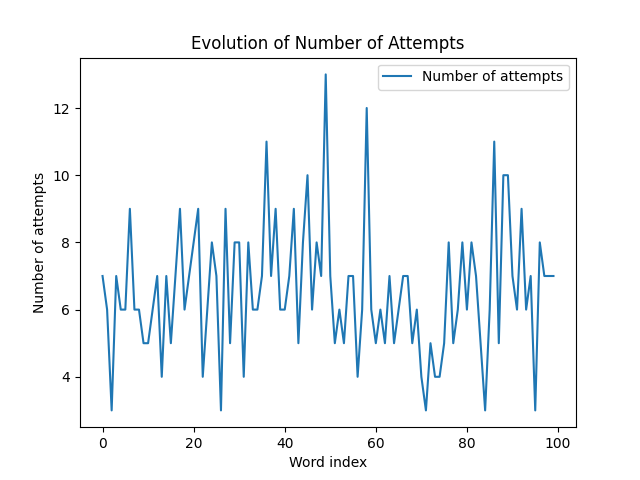
\includegraphics[scale=0.7]{images/start1.png}
\caption{100 first words, for start word 1 (50\% win rate)}
\label{start1}
\end{figure}

\begin{figure}[!h]
\centering
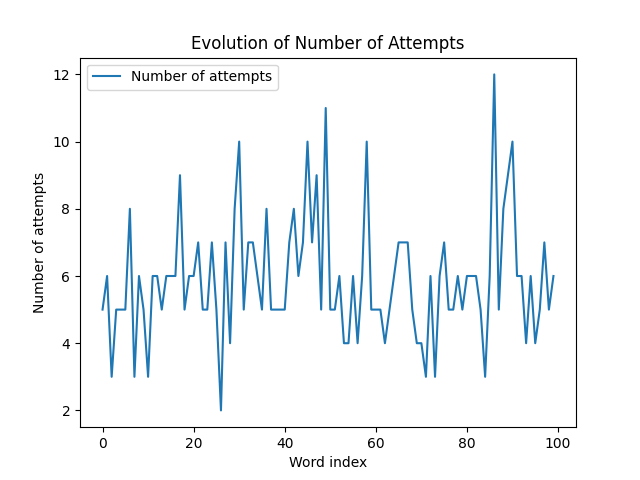
\includegraphics[scale=0.7]{images/start2.png}
\caption{100 first words, for start word 2 (70\% win rate)}
\label{start2}
\end{figure}

\newpage

It's obvious that the second "first word technique" is the best, giving approximately 70\% of win, against 50\% for the first. (we didn't implement the third)

\begin{figure}[!h]
\centering
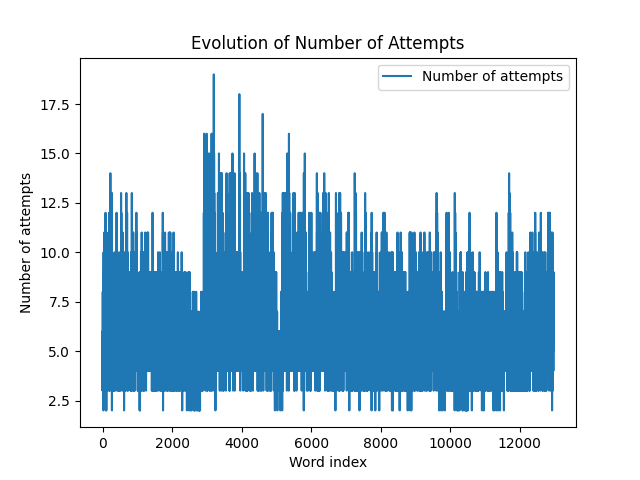
\includegraphics[scale=0.7]{images/start2-total.png}
\caption{all words in list, for start word 2}
\label{total}
\end{figure}

Note that these comparisons and calculations are based on the given list of 5-letter words. An interesting approach would have been to have the same statistics but on the whole English language. In this way, the frequencies of symbols and "blocks" of symbols would not be the same.

Once it has the best first word, the bot will sort the list of possible words according to feedback, then play the word with the highest entropy from this list. 